\part{Using LabPlot}

\chapter{Interface}
\section{Main Area}
\section{Project Explorer}
\section{Properties Explorer}

\chapter{Data Containers}
\section{Spreadsheet}
\section{Matrix}
\section{Workbook}

\chapter{2D Plotting}
\section{Plots}
\section{Curves}
\section{Legends}


% \chapter{3D Plotting}

\chapter{Themes and Templates}


\chapter{Data Analysis}
\section{Data reduction}
\section{Differentiation}
\section{Integration}
\section{Interpolation}
\section{Smoothing}
\section{Curve Fitting}
\section{Fourier Filter}
\section{Fourier Fransform}

\chapter{CAS Computing}
LabPlot can be used as a frontend to different open-source computer algebra systems (CAS) like Maxima, Octave, R, Scilab and Sage  or programming languages providing similar capabilities like Python and Julia. LabPlot recognizes different CAS variables holding array-like data and allows to select them as the source for curves. So, instead of providing columns of a spreadsheet as the source for x- and y-data, the user provides the names of the corresponding CAS-variables. Currently supported CAS data containers are
\begin{itemize}
\item \textbf{Maxima} lists
\item \textbf{Python} lists, tuples and NumPy arrays
\item \textbf{Julia} vectors and tuples
\end{itemize}

With this, powerfull calculations carried out inside of different CAS environments can be combined with the user-friendly visualisation and editing capabilities of LabPlot. This combination is demonstrated below with the help of two examples:
\begin{figure}
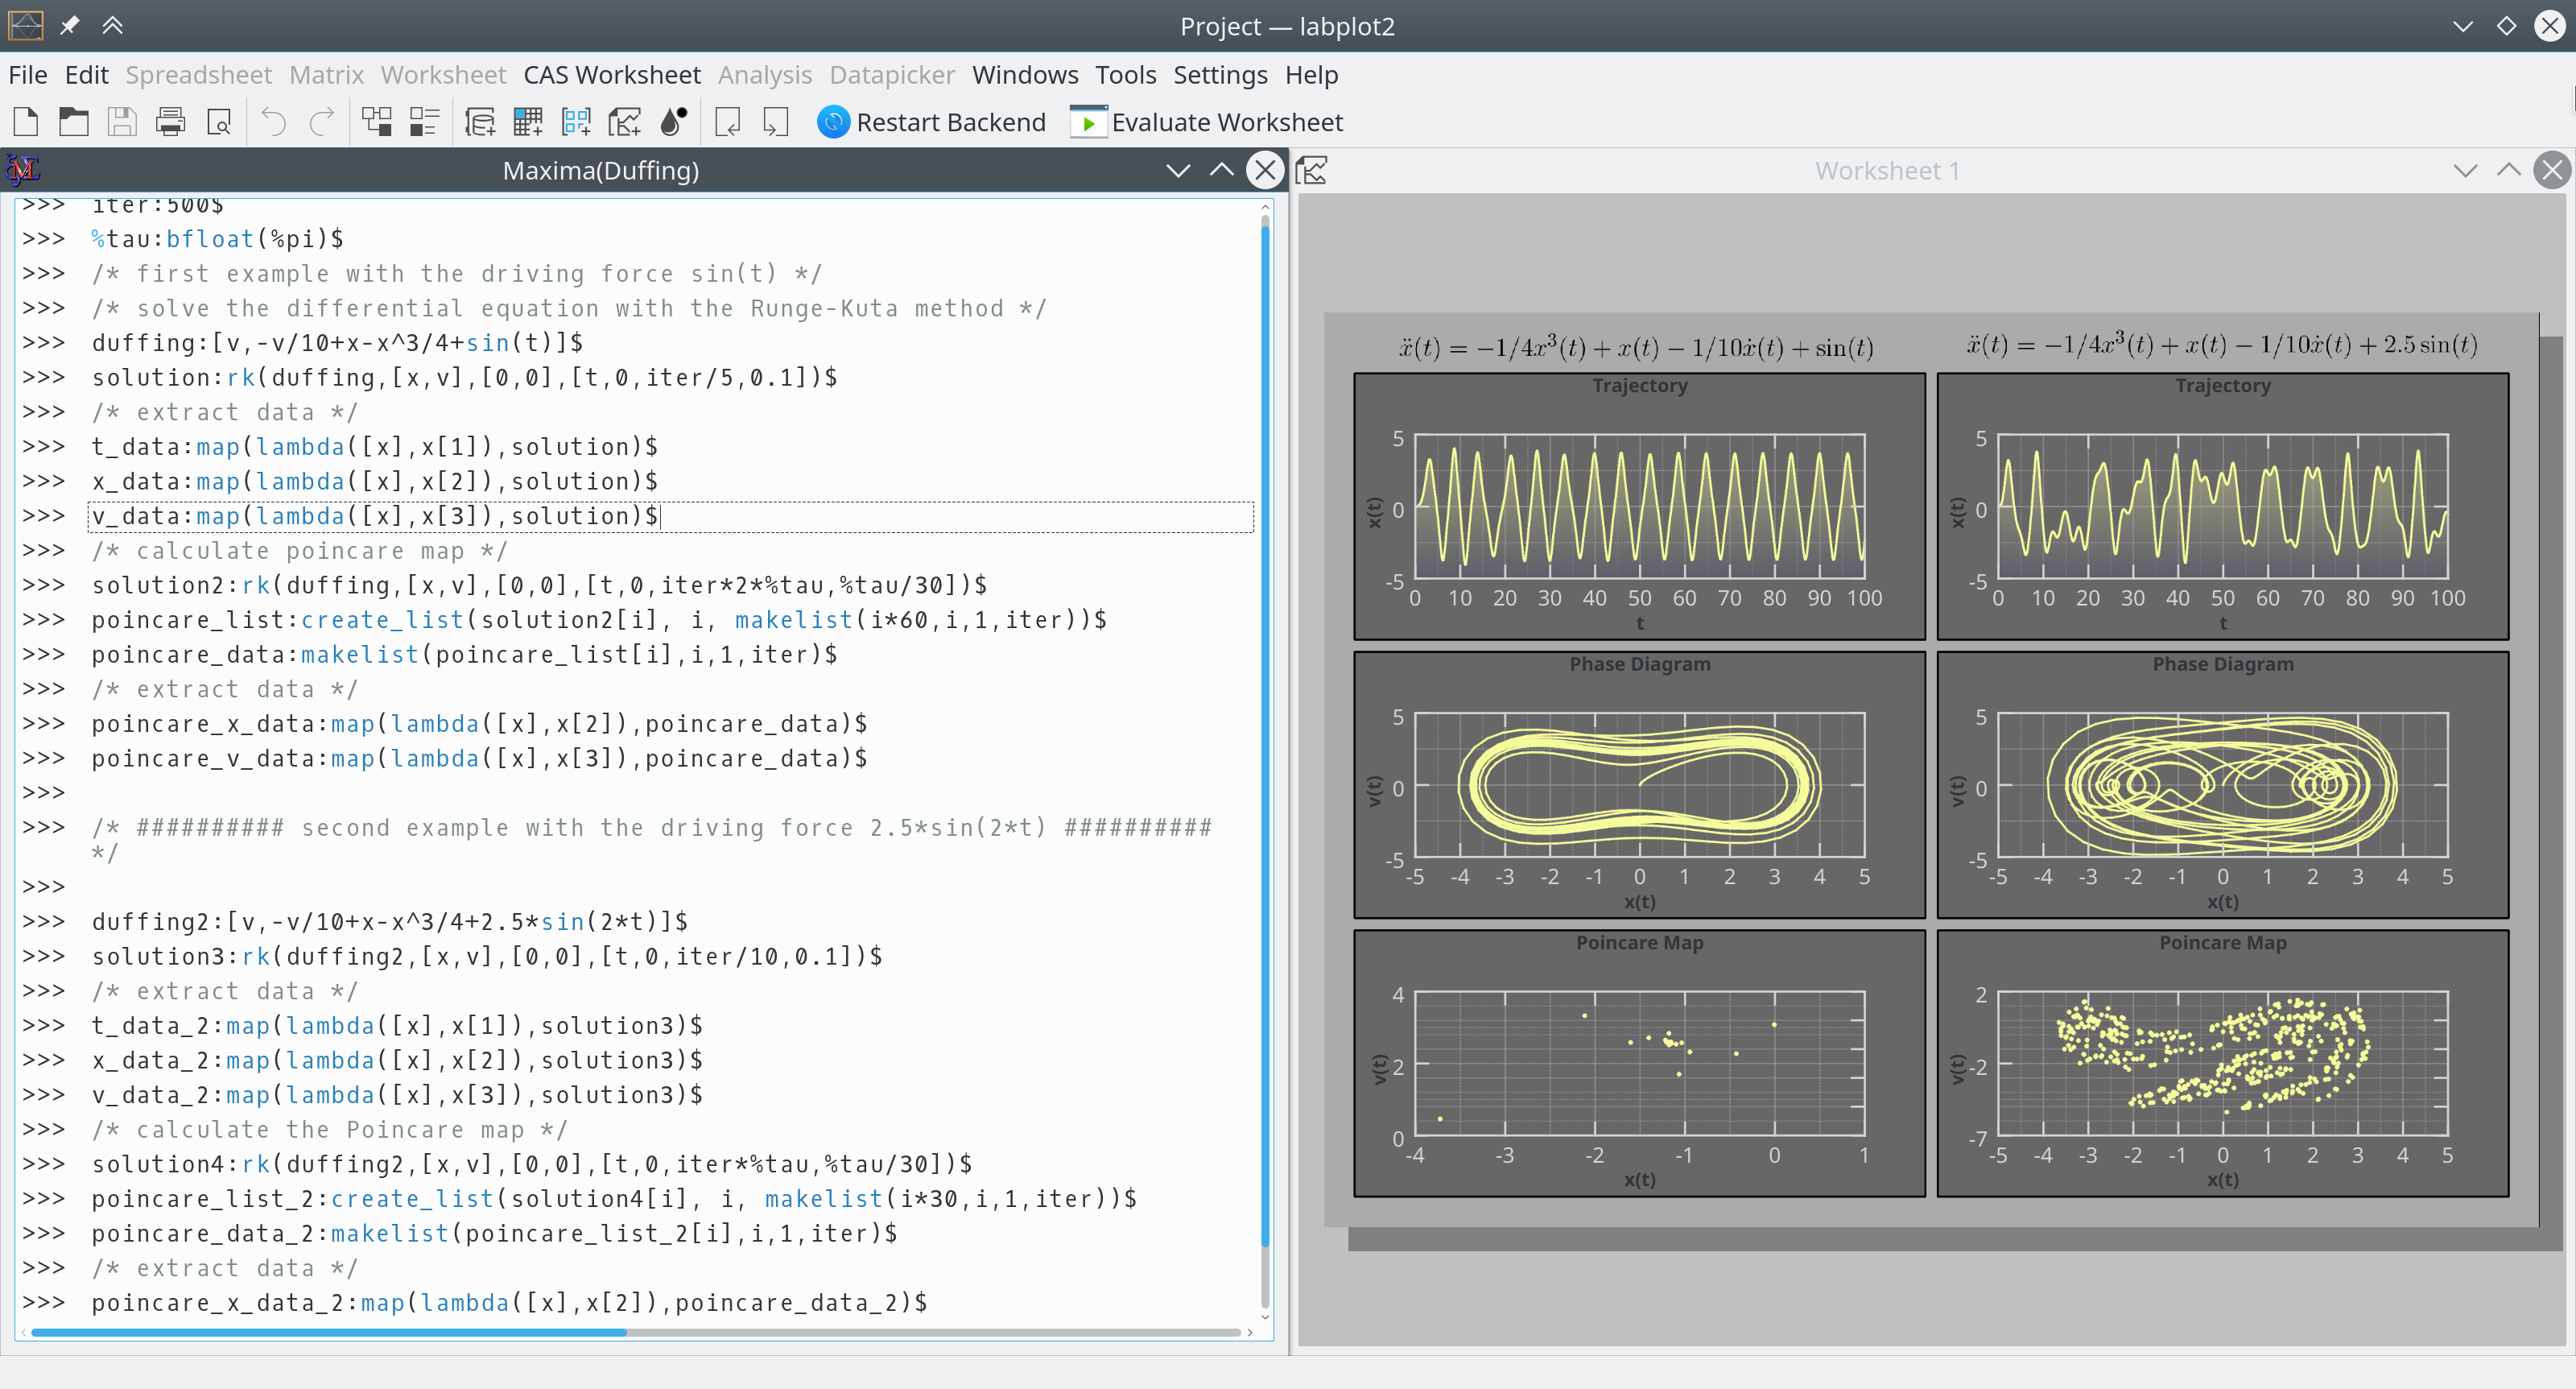
\includegraphics[width=\textwidth]{images/maxima_session.png}
\caption{Maxima session showing the chaotic dynamics of the Duffing oscillator. The differential equation of the forced oscillator is solved with Maxima. Plots of the trajectory, the phase space of the oscillator and the corresponding Poincaré map are done with LabPlot.}
\end{figure}

\begin{figure}
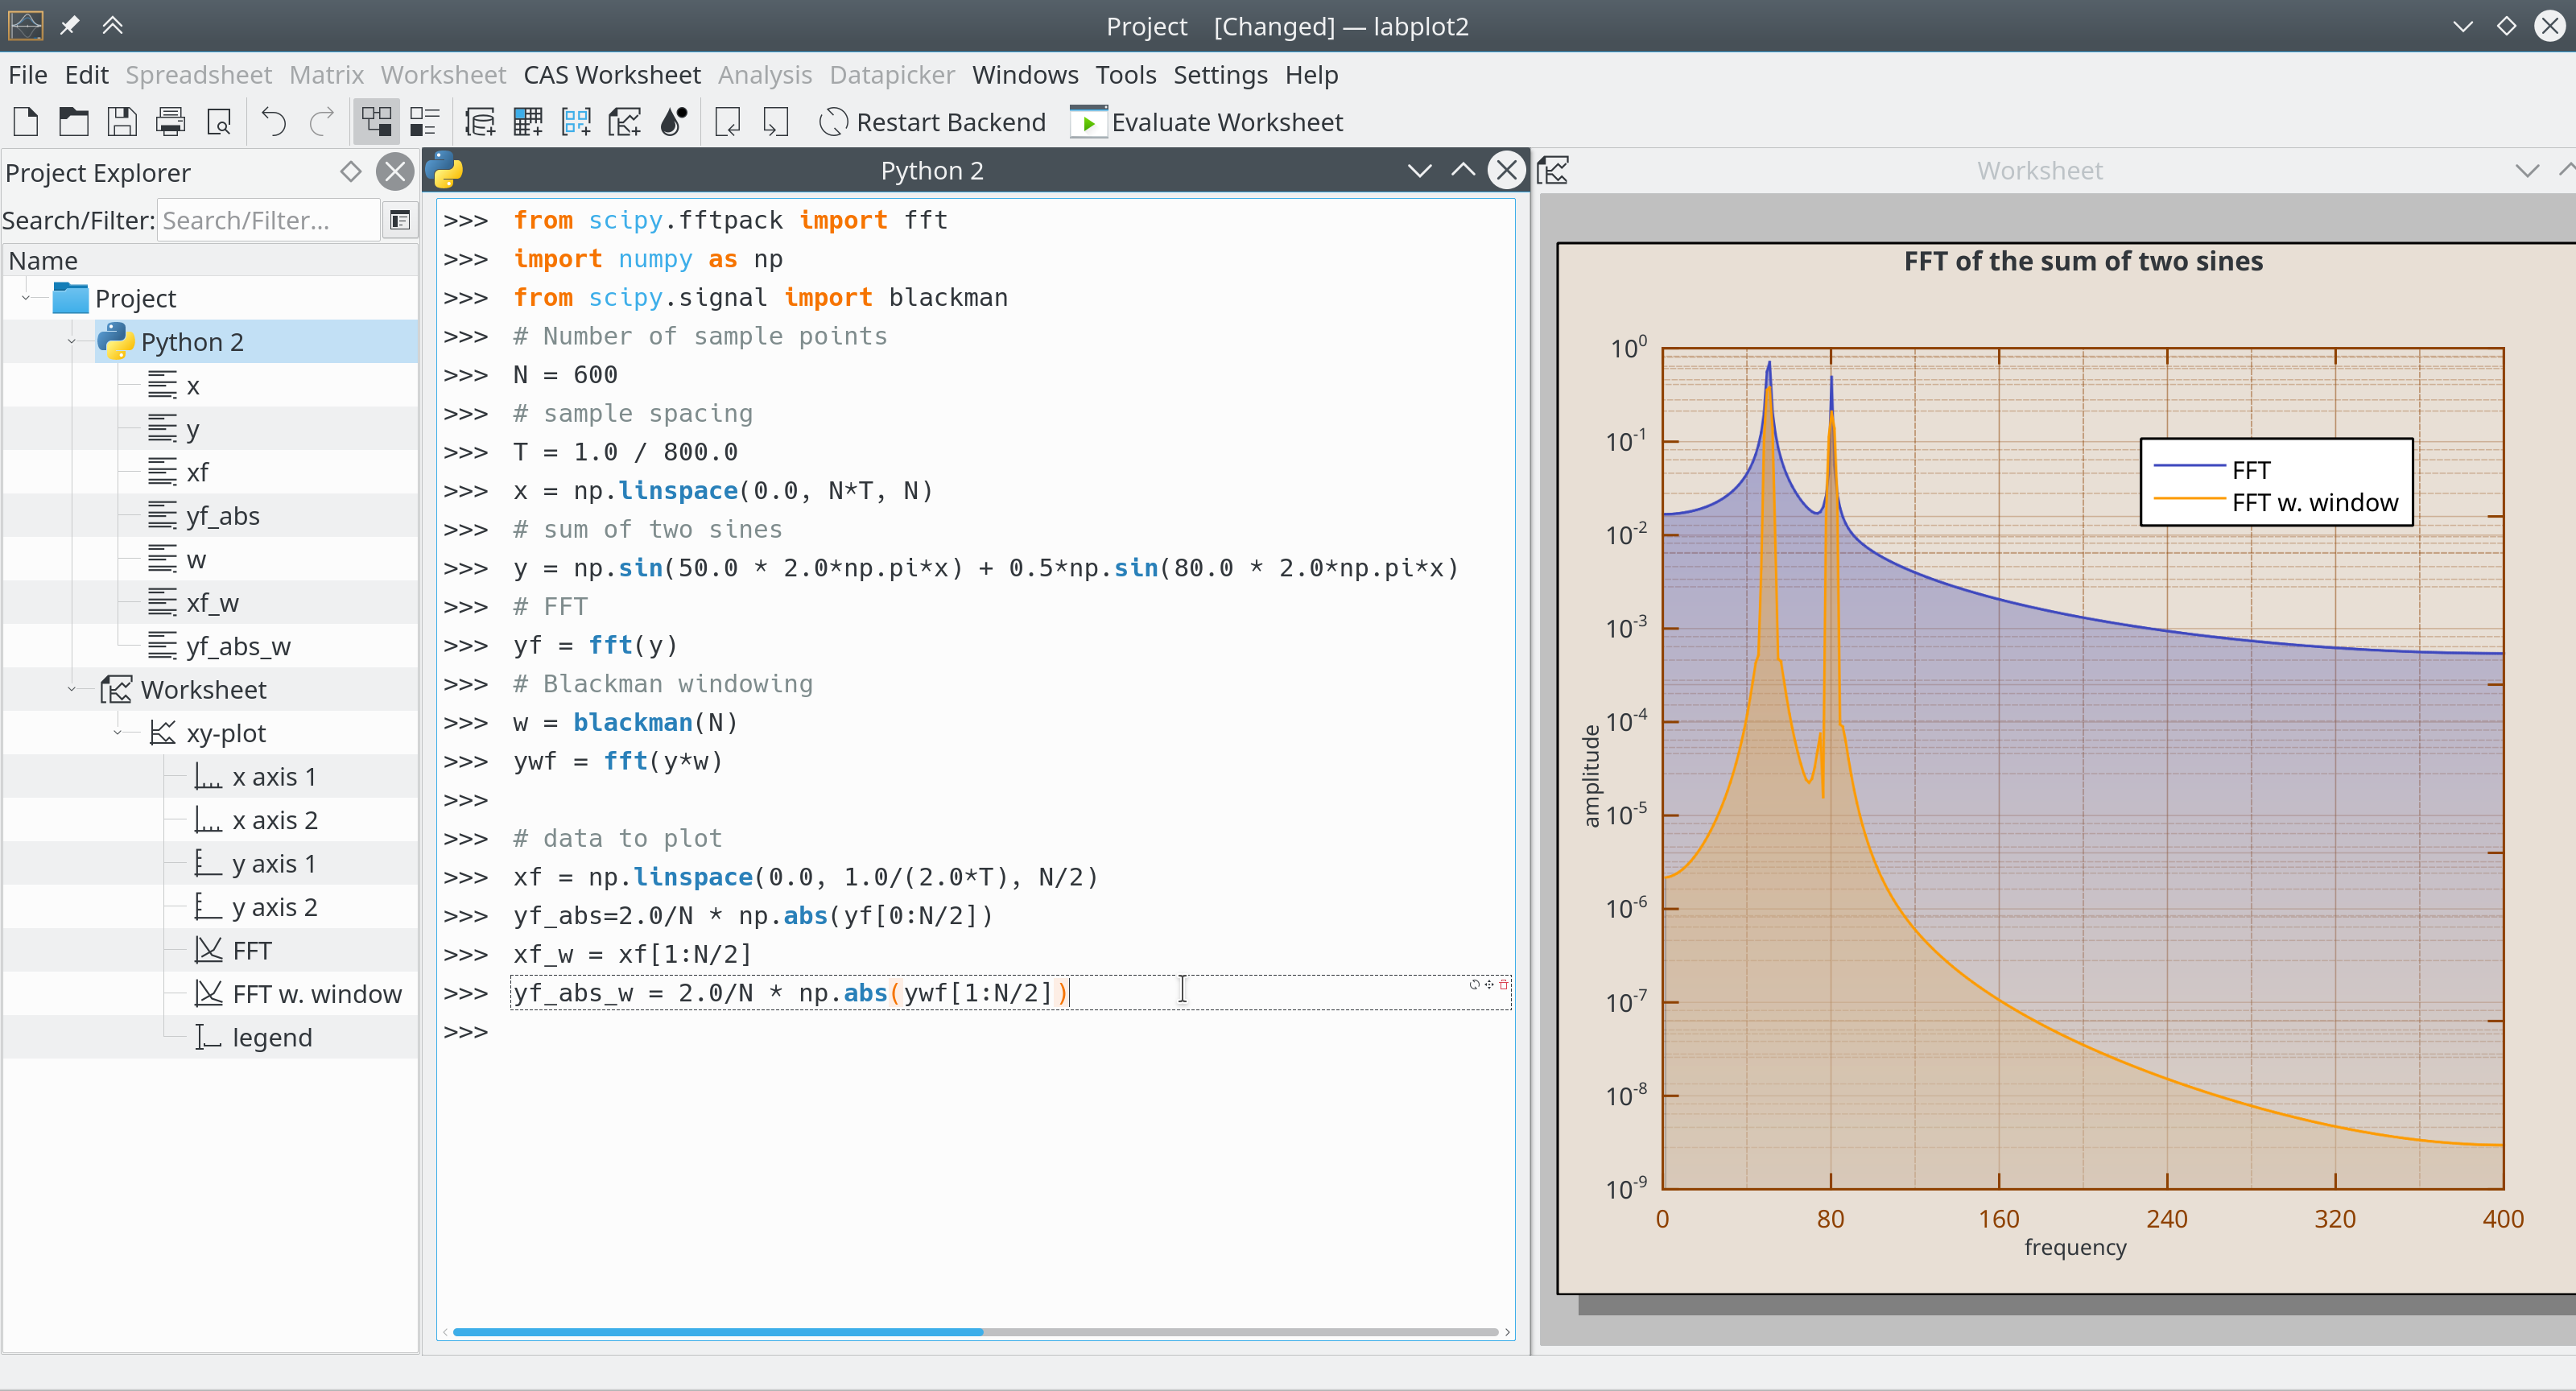
\includegraphics[width=\textwidth]{images/python_session.png}
\caption{Python session illustrating the effect of Blackman windowing on the Fourier transform:}
\end{figure}



\chapter{Import and Export}
\section{Import}
\section{Export}

\chapter{Latex Typesetting}

\chapter{Tools}
\section{Curve Tracing}
\section{FITS Metadata Editor}
